%% 
%% Copyright 2007-2024 Elsevier Ltd
%% 
%% This file is part of the 'Elsarticle Bundle'.
%% ---------------------------------------------
%% 
%% It may be distributed under the conditions of the LaTeX Project Public
%% License, either version 1.3 of this license or (at your option) any
%% later version.  The latest version of this license is in
%%    http://www.latex-project.org/lppl.txt
%% and version 1.3 or later is part of all distributions of LaTeX
%% version 1999/12/01 or later.
%% 
%% The list of all files belonging to the 'Elsarticle Bundle' is
%% given in the file `manifest.txt'.
%% 
%% Template article for Elsevier's document class `elsarticle'
%% with numbered style bibliographic references
%% SP 2008/03/01
%% $Id: elsarticle-template-num.tex 249 2024-04-06 10:51:24Z rishi $
%%
%\documentclass[preprint,12pt]{elsarticle}
\documentclass[5p,,preprint,12pt]{elsarticle}

%% Use the option review to obtain double line spacing
% \documentclass[authoryear,preprint,review,12pt]{elsarticle}

%% Use the options 1p,twocolumn; 3p; 3p,twocolumn; 5p; or 5p,twocolumn
%% for a journal layout:
% \documentclass[final,1p,times]{elsarticle}
% \documentclass[final,1p,times,twocolumn]{elsarticle}
% \documentclass[final,3p,times]{elsarticle}
%\documentclass[final,3p,times,twocolumn]{elsarticle}
% \documentclass[final,5p,times]{elsarticle}
% \documentclass[final,5p,times,twocolumn]{elsarticle}

%% For including figures, graphicx.sty has been loaded in
%% elsarticle.cls. If you prefer to use the old commands
%% please give \usepackage{epsfig}

%% The amssymb package provides various useful mathematical symbols
\usepackage{amssymb}
%% The amsmath package provides various useful equation environments.
\usepackage{amsmath}
\usepackage{url,multirow,morefloats,floatflt,cancel,tfrupee}
\usepackage{tabulary,xcolor}
\usepackage{amsfonts,amsmath}
\usepackage[T1]{fontenc}
\usepackage{graphicx}

%% The amsthm package provides extended theorem environments
%% \usepackage{amsthm}

%% The lineno packages adds line numbers. Start line numbering with
%% \begin{linenumbers}, end it with \end{linenumbers}. Or switch it on
%% for the whole article with \linenumbers.
%% \usepackage{lineno}

\journal{Computers in Biology and Medicine}

\begin{document}

\begin{frontmatter}

%% Title, authors and addresses

%% use the tnoteref command within \title for footnotes;
%% use the tnotetext command for theassociated footnote;
%% use the fnref command within \author or \affiliation for footnotes;
%% use the fntext command for theassociated footnote;
%% use the corref command within \author for corresponding author footnotes;
%% use the cortext command for theassociated footnote;
%% use the ead command for the email address,
%% and the form \ead[url] for the home page:

%% \title{Title\tnoteref{label1}}
%% \tnotetext[label1]{}
\author[1,2]{Duc-Tinh Pham}
%\ead{tinhpd@haui.edu.vn}
%\ead[url]{www.haui.edu.vn}

\affiliation[1]{organization={Complex Systems and Bioinformatics Lab, Hanoi University of Industry},
            addressline={298 Cau Dien Street, Bac Tu Liem District},
            city={Hanoi},
          %  postcode={10000},
           % state={},
                 country={Vietnam}}

 \author[1,3]{Tien-Dzung Tran \corref{cor1}}
 \ead{trantd@haui.edu.vn}
 \ead[url]{www.haui.edu.vn}
% \fntext[label2]{This research was funded by Hanoi University of Industry.}
 \cortext[cor1]{Corresponding author.}
 
\affiliation[2]{organization={Gruduate University of Science and Technology, Academy of Science and Technology Vietnam},
             addressline={18 Hoang Quoc Viet Street, Cau Giay Distris},
             city={Hanoi},
           % postcode={10000},
           % state={},
            country={Vietnam}}
            
\affiliation[3]{organization={Faculty of Information and Communication Technology, Hanoi University of Industry},
            	addressline={298 Cau Dien Street, Bac Tu Liem District},
            	city={Hanoi},
            %	postcode={10000},
            %	state={},
            	country={Vietnam}}
%% \fntext[label3]{}

\title{\textbf{Drivergene.net: A Cytoscape app for the identification of driver nodes of large-scale complex networks and case studies in discovery of drug target genes.}}

%% use optional labels to link authors explicitly to addresses:

 
%% Author affiliation

            
%% Abstract
\begin{abstract}
%% Text of abstract
There are no tools to identify driver nodes of large-scale networks in approach of competition-based controllability. This study proposed a novel method for this computation of large-scale networks. It implemented the method in a new Cytoscape plug-in app called Drivergene.net. Experiments of the software on large-scale biomolecular networks have shown outstanding speed and computing power. Interestingly, 86.67\% of the top 10 driver nodes found on these networks are anticancer drug target genes that reside mostly at the innermost K-cores of the networks. Finally, compared method with those of five other researchers and confirmed that the proposed method outperforms the other methods on identification of anticancer drug target genes. Taken together, Drivergene.net is a reliable tool that efficiently detects not only drug target genes from biomolecular networks but also driver nodes of large-scale complex networks. Drivergene.net with a user manual and example datasets are available https://github.com/tinhpd/Drivergene.git
\end{abstract}

%%Graphical abstract
%\begin{graphicalabstract}
%\includegraphics{grabs}
%\fixFloatSize{images/abstract}
%\end{graphicalabstract}

%%Research highlights
%\begin{highlights}
%\item Research highlight 1
%\item Research highlight 2
%\end{highlights}

%% Keywords
\begin{keyword}
%% keywords here, in the form: keyword \sep keyword

%% PACS codes here, in the form: \PACS code \sep code

%% MSC codes here, in the form: \MSC code \sep code
%% or \MSC[2008] code \sep code (2000 is the default)
Drug target genes\sep Competitive dynamics model\sep Complex network\sep Cytoscape plug\-in\sep Driver node identification
\end{keyword}

\end{frontmatter}

%% Add \usepackage{lineno} before \begin{document} and uncomment 
%% following line to enable line numbers
%% \linenumbers

%% main text
%%

%% Use \section commands to start a section
\section{Introduction}
The identification of driver nodes in complex networks has been a topic of significant research in the field of network science. Several scientific and applied achievements have contributed for understanding this important aspect of network control. First, Liu et al. investigated the concept of structural controllability in linear complex networks \cite{1}. They demonstrated that the minimum set of driver nodes, which can control the network, can be computed efficiently using a reduction to the maximum matching problem on bipartite graphs. This work laid the foundation for subsequent studies on driver node identification. Building upon Liu et al.'s findings, Ruths and Ruths explored the maximum matching approach in network controllability and classified control profiles based on different types of controls, such as swece nodes, external dilations, and internal dilations \cite{2}. Their work provided insights into the diversity of control mechanisms in complex networks. Besides, Nepusz and Vicsek focused on controlling edge dynamics in complex networks \cite{3}. They proposed a method to identify the optimal set of driver nodes using the concept of the region of attraction. Their approach offered a new perspective on achieving control in complex networked systems. In a study by Wei et al., a practical problem called the target control problem with objectives-guided optimization (TCO) was addressed \cite{4}. The goal was to control specific variables or targets in a network while minimizing the number of driver nodes and maximizing the quantity of constrained nodes. They developed an efficient algorithm called TCOA, which outperformed existing control-focused approaches in identifying precise driver nodes. These publications have significantly advanced the understanding of driver node identification in complex networks, but their methods were based on network structure, which may be ineffective with networks with similar structure but different in dynamics. Recently, Tran et al proposed a dynamics model to identify driver nodes based on the simulation of a competition between inside agents and an outside agent where driver nodes are the inside nodes with the highest total support score receiving from the other nodes \cite{5}. The suty  applied the model to 17 different cancer signaling networks and found that driver nodes are often anticancer drug target genes. This result confirmed the precision of the dynamics model and shows the potential of driver nodes in the identification of therapeutic targets in drug discovery. The discovery of anticancer drug target genes is an important step in the development of drugs to treat cancer. Therefore, it is extremely important to develop tools that can accurately identify anticancer drug target genes. In recent years, several tools have been introduced to identify anticancer drug target genes. These tools can be categorized into three main approaches: machine learning-based methods, mutation similarity-based statistics methods, and network-based methods.\\
Machine learning-based methods involve the use of supervised machine learning technology to identify anticancer drug target genes. Examples of such tools include DriverML, which quantifies the functional impacts of mutations on proteins to identify target genes \cite{6}, and EARN (Ensemble of Artificial Neural Network, Random Forest, and non-linear Support Vector Machine), which uses machine learning to evaluate metastasis breast anticancer drug target genes \cite{7}. Another tool called PCDG-Pred distinguishes the attributes of anticancer drug target genes from passenger attributes using genomic sequencing data and a machine learning model \cite{8}. However, a limitation of this approach is the requirement for large sample sets and standardized anticancer drug target gene datasets, which may not be available for every cancer type \cite{9}. \\
Mutation similarity-based statistics methods focus on evaluating mutations and their similarity to identify anticancer drug target genes. DrGaP is a versatile tool that identifies anticancer drug target genes and controls signaling pathways in gene-based sequencers \cite{10}. OncodriveCLUST is another method that identifies target genes by evaluating noncoding mutations from somatic mutations \cite{11}. OncoVar utilizes known bioinformatics algorithms to identify target genes based on the oncogenic potential of somatic mutations and cancer genes \cite{12}. A limitation of this approach arises when known and unknown disease genes have indirect relationships or similar functions, leading to incorrect function annotation and affecting prediction results \cite{13,14}. \\
The network-based approach considers the observation that genes associated with the same or similar diseases tend to be located close together in biomolecular networks \cite{15}. This approach can be divided into two groups: local methods and global methods \cite{16}. Local methods focus on genes that are directly connected or have the shortest path to the identified causative genes \cite{17,18,19,20,21,22,23,24,25}. Global methods utilize algorithms to propagate disease information from known disease genes through a network system and assign candidate gene weights based on similarity to known disease genes \cite{26,27,28}. Network-based studies require less data but need improvement in accuracy. \\
Here, based on dynamic network model, namely outside competitive dynamics model, the study proved that driver nodes can identify anticancer drug target genes \cite{5}. However, the algorithm works inefficiently on large-scale networks, so it can not discover insights from these large networks. In other words, controllability characteristics of large-scale complex network is still in mystery because of no analysis tool for them. In this study, the study proposed a new version of parallel algorithm to effectively execute on large-scale molecular biological networks. In addition, a new software tool was developed for integration into Cytoscape, called Drivergene.net, which implements the outside competitive dynamic model with the parallel algorithm using the OpenCL library in Java to ensure that the algorithm is scalable on large-scale biomolecular networks. The library utilizes the full computing power of a multi-core central processing unit \cite{29,30}, enabling more efficient in the computational performance of the software. The software is developed as a Cytoscape plug-in with a user-friendly graphical user interface (GUI) where network visualization functions, necessary data, and options are easily set through the GUI of Cytoscape. To test the computational performance of Drivergene.net for identifying driver nodes in large-scale biomolecular networks, the study performed an analysis of three large-scale biomolecular networks, including: human signaling network, human protein-protein interaction network, and human gene regulatory network. The results showed that parallel execution for multi-core CPUs provides a maximum acceleration factor that outperforms sequential computations on single core CPUs. In particular, 86.67\% of the top 10 driver genes with the highest total support score computed by Drivergene.net were in fact anticancer drug target genes in cancer therapy. In addition, these genes were mostly within the innermost core of the networks. This finding is in agreement with the results of previous studies that important cancer biomarker genes are often located in the innermost core of the biological network \cite{31,32,33,34}, and anticancer drug target genes often act as target genes for cancer drugs and cancer biomarker genes in the biological networks \cite{23}. Finally, to evaluate the prediction results on anticancer drug target genes, the sudy made a comparison between the results of Drivergene.net with those of five other methods based on earlier work in this area. As a result, Drivergene.net's predictions for the three networks exhibited a better result than those of the previous methods because sharing the largest number of anticancer drug target genes crossing. This comparison result showed that the genes found from the networks share consensus with those found by other studies and that the method of Drivergene.net is better than other methods. Drivergene.net is a reliable tool that efficiently detects not only anticancer drug target genes from biomolecular networks but also driver nodes of large-scale complex networks.

\section{Methods and Materials}
\subsection{Experimental Data } 
The study utilized data from three previously publications. The first network is a human signaling network \cite{18}, containing 1561 nodes and 5089 edges, including 2403 activating edges labeled as +1, 741 inhibiting edges labeled as -1, 1915 neutral edges labeled as 0, and 30 edges of unknown type, labeled as 0. This network was manually constructed and their interactions were derived from the comprehensive signaling pathway database BioCarta (http://www.biocarta.com/). Pathways in the database are illustrated as diagrams manually constructed. To ensure the accuracy of interactions, all data underwent four-fold cross-checking by different researchers. Subsequently, the network was further expanded by integrating interactions from the Cancer Cell Map (http://cancer.cellmap.org/cellmap/), a database containing 10 manually curated signaling pathways for cancer. \\
The second network is a large-scale human protein-protein interaction network downloaded from \cite{19}. The network contains 7533 nodes and 22052 edges, generated through high-throughput techniques of protein - protein interactions at the genome scale, combining two-hybrid experiments to identify binary interactions. \\
The third network is a human gene regulatory network containing 943 genes and 3922 edges, introduced in \cite{20}. The dataset was built from knowledge of gene regulatory networks by collecting and integrating the regulatory interactions between transcription factors (TFs), microRNAs (miRNAs), and the target genes from 25 databases. The result is a dataset containing a comprehensive set of regulatory interactions. Furthermore, the study also describes statistical properties and structural characteristics of regulatory gene networks across the entire human genome, extracting and explaining important networks related to interactions between TF-miRNA and their targets. 

\begin{figure*}[!ht]
	\centering 
	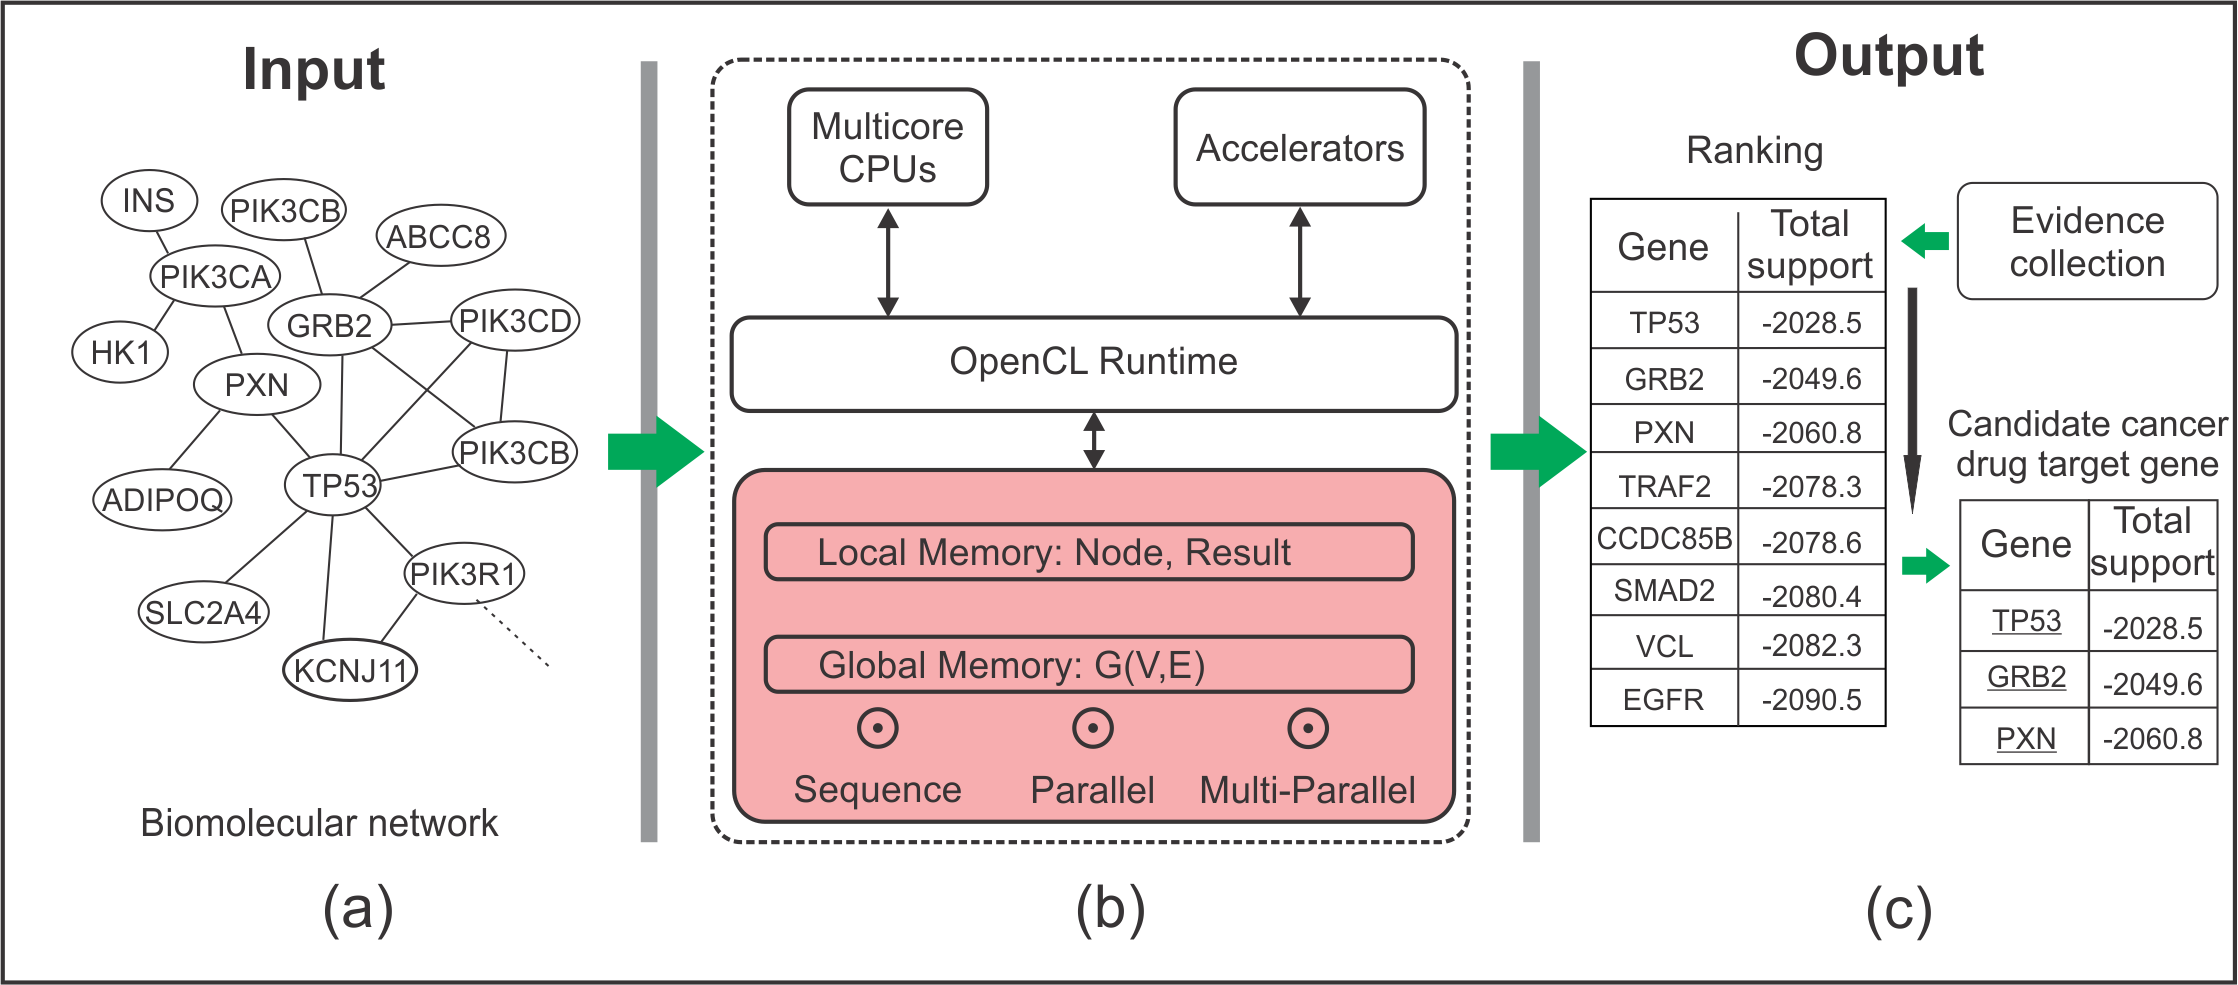
\includegraphics[scale=0.95]{images/fig1.png}
	\caption{The design of Drivergene.net to identify driver nodes of a complex network.}
	\label{figure-1}
\end{figure*}

Figure 1a, Network preprocessor module. The input data network is a complex network, and this module converts various network types into a single network. Figure 1b,  Analysis module. The main module of Drivergene.net is developed using an outside competitive dynamics model that identifies driver nodes, with the highest total support, of the network. The parallel algorithm is used with the help of the OpenCL library to ensure the algorithm's scalability on large-scale networks. Figure 1c, The presenting module. The output data is a list of nodes ranked by total support in descending order. With the help of evidence collected from PubMed, the driver nodes are often anticancer drug target genes in biomolecular networks.

\subsection{Design and implementation}
The study propose a software design for identifying driver nodes of a complex network, which often are anticancer drug target genes on large-scale molecular biological networks. This software exploited the outside competitive network dynamic model that was introduced in the previous study \cite{5}. The software architecture includes three modules (Figure 1). First, the network preprocessor module (Figure 1a) is used to obtain input data and convert various network types into a single network, after extracting the maximum connected components of the network. Second, the analysis module (Figure 1b) with the outside competition dynamic model \cite{5} integrated to determine the driver nodes of the disease network \cite{23}, with a parallel computing technique being applied and the help of the installed OpenCL library. This is a solution that fully exploits the computing resource of multi-core processors because it uses the OpenCL library which is designed to run on any available multi-core CPU. Next, the application computes the total support of each node in the network. In turn, each thread loads and processes a selected amount of network data, in relation to the settings of the respective algorithm. The native source code supports connection and data processing and plays an intermediary role in converting the source code to OpenCL and processing on CPUs. It loads the data, converted into an array, into the kernel and then initializes the local area of the memory to load data into the CPU cores for processing. Third, the presenting module (Figure 1c) creates the output of the computation as a list of genes in the network and ranks nodes in descending order by total support. Finally, biomedical evidence is collected from the PubMed database for the top 10 highest-ranking genes used.

\subsection{Parallel algorithms for the identification of driver nodes with OpenCL}
Next, using the mathematical model of the outside competitive network dynamics model, the study designed a parallel version of the algorithm published previously and implemented this version with the help of the OpenCL library installed. 
The algorithm in Algorithm 1 has the main entry as \textit{ParFindDriverNode} which parallelly calls \textit{ToS} sub-function for computing total support of every node. The \textit{OutsideCompetition} sub-function is called by \textit{ToS} to calculate influence of vertices in the network with a specific vertex $\alpha$ as the driver when an outside agent $\beta$ is present. This function includes initializing the initial state of the vertices, creating a connection with the outside agent, updating the state of the vertices in the network by \textit{InsideCompetition} sub-function, and checking the stopped condition of the algorithm. The output of this sub-function is the supporting score of the other nodes to driver $\alpha$. For each vertex $\alpha$ traversed, \textit{ParFindDriverNode} calls the \textit{ToS} to determine whether a vertex $\alpha$ is a driver or not by checking their total support score to reach the highest value.
\textbf{Algorithm 1}. Parallelly finding driver nodes of a complex network G(V, E). This algorithm is applied in the identification of anticancer drug target genes from biomolecular networks. \\
\textbf{function} \textit{$[X_t]$ InsideCompetition(G(V,E), Leaders $\in$ V,AgainstLeaders $\in$ V)}  \\
\textit{maxIterations $\gets$ V $\times$ E; \textit{Epsilon} $\gets$  4.94e-324;}  \\
\textit{$\varepsilon \gets$ 1/(Max(total weights of out-links of v, $\forall$v $\in$V) - Epsilon}; \\
\textit{$X_t$} $\gets$ \textbf{new} \textit{Dictionary(node,value); $X_{t+1}$ $\gets$} \textbf{new} \textit{Dictionary(node,value);} \\
\textbf{for} (\textit{Node} \textbf{in} \textit{V} ) \textbf{do} \\
\hspace{0.5cm}   \textit{$X_t$[Node] $\gets$ 0;} \textbf{end for} \\
\textbf{for} (\textit{Leader} \textbf{in} \textit{Leaders}) \textbf{do} \\
\hspace{0.5cm} \textit{$X_t$[Leader] $\gets$ 1; $X_{t+1}$[Leader] $\gets$ 1;} \textbf{end for} \\
\textbf{for} (\textit{AgainstLeader} \textbf{in} \textit{AgainstLeaders}) \textbf{do} \\
\hspace{0.5cm} \textit{$X_t$[AgainstLeader] $\gets$ -1; $X_{t+1}$[AgainstLeader] $\gets$ -1};
\textbf{end for} \\
\textit{Error $\gets$ 0; t $\gets$ 0};  \\
\textbf{Do} \\
\hspace{0.5cm} \textit{Error $\gets$ 0}; \\
\hspace{0.5cm} \textbf{for} (\textit{u} \textbf{in} \textit{V}) \textbf{do}  \\
\hspace{1cm}  \textbf{if} (\textit{Leaders contain u} \textbf{or} \textit{AgainstLeaders contain u}) \textbf{continue; end if} \\
\hspace{1cm} \textit{r $\gets$ 0} \\
\hspace{1cm} \textbf{for} (\textit{v} \textbf{in} \textit{Neighbors of u}) \textbf{do} \\
\hspace{1.5cm} \textit{r $\gets$ r} + \textit{weight(u,v)} $\times$ \textit{($X_t$[v] - $X_t$[u])}; \textbf{end for} \\
\hspace{1cm} \textit{$X_{t+1}$[u] $\gets$ $X_t$[u]} + $\varepsilon$ $\times$ \textit{r}; \\
\hspace{1cm} \textit{Error $\gets$ Error} + \textit{Math.Abs($X_t$[u]} - \textit{$X_{t+1}$[u]}); \\
\hspace{0.5cm} \textbf{end for;} \\
\hspace{0.5cm}  \textit{Temp $\gets$ $X_t$; $X_t$ $\gets$ $X_{t+1}$; $X_{t+1}$ $\gets$ Temp}; \textit{t $\gets$ t}+\textit{1}; \\
\textbf{while} (\textit{Error}  $>$ \textit{Epsilon} $\land$ t $<$ \textit{maxIterations)}; \\
\textbf{return} \textit{$X_t$}; //Output as stable states of nodes as t $\to$ $\infty$ \\
\textbf{end} \\
\textbf{function} \textit{[Support] OutsideCompetition (G(V,E), $\alpha$ $\in$ V}) \\
\textit{Support} $\gets$ \textbf{new} \textit{Dictionary(node,value)}; \\
$\beta$ $\gets$ \textbf{new} \textit{Node}; \\
\textit{NormalAgents $\gets$ V $\setminus$ \{$\beta$, $\alpha$\}}; \\
\textbf{for} ($\gamma$ \textbf{in}  \textit{NormalAgents} ) \textbf{do}   \\
\hspace{0.5cm}  \textit{e} $\gets$ \textbf{new} \textit{Edge($\beta$, $\gamma$)}; \textit{E= E $\cup$ e}; \\
\hspace{0.5cm}  \underline{X} $\gets$ \textit{InsideCompetition(G(V,E)}, $\alpha$,$\beta$); \\
\textit{Support[$\gamma$] $\gets$  \underline{X}[$\gamma$]; E= E $\setminus$ e}; \textbf{end for} \\ 
\textbf{return} \textit{Support}; //Support of nodes to $\alpha$ when connecting to $\beta$ \\
\textbf{end} \\
\textbf{procedure} \textit{ToS(G(V,E), $\alpha$ $\in$ V}, \textbf{out}     \textit{result}) \\
\textit{Support} $\gets$ \textbf{new} \textit{Dictionary(node,value)}; \\
\textit{Support $\gets$ OutsideCompetition (G(V,E), $\alpha$)}; \\
\textit{TotalSupport $\gets$ 0}; \\
\textbf{for}($\gamma$ \textbf{in} \textit{V} $\setminus$ $\alpha$) \textbf{do} \\
\hspace{0.5cm}  \textit{TotalSupport $\gets$  TotalSupport} + \textit{Support[$\gamma$]}; \\
\textbf{end for} \\
\textit{result[$\alpha$]}= \textit{TotalSupport}; //Total support of nodes to $\alpha$ \\
\textbf{end} \\
\textbf{function} \textit{[driver nodes]} \textit{ParFindDriverNode(G(V,E))} \\
\textit{//G(V,E)}: Global variable; \textit{$\alpha$}: Local variable; \textit{result}: Local variable; \\
\textit{result} $\gets$ \textbf{new} \textit{Dictionary(node,value)}; \\
\textbf{for}($\alpha$ \textbf{in} \textit{V}) \textbf{in parallel do} \\
\hspace{0.5cm}  \textit{ToS(G(V,E)},$\alpha$, \textit{result}); \\
Wait for all works done();\textbf{ end for} \\
\textbf{return} \textit{result with the highest total support score}; \\
\textbf{end.} 

\section{Results}
\subsection{Drivergne.net app in Cytoscape}
Drivergene.net is developed in a Java programming environment with using the availability of OpenCL library installed as a solution that fully exploits the computing power of multi-core CPUs. The software was compiled and packaged separately as a plug-in for Cytoscape, and can be run on any system where Java Virtual Machine is installed, including Windows, Ubuntu, and Mac OS. The user can choose the network data and execution among many options, such as executing in sequential on CPU, executing in parallel on CPUs, or executing in parallel on all computing devices. The user can flexibly provide input network data and get output computation results according to the data standards supported by Cytoscape. The software works with three main functions, including 1) Visualizing the network, 2) Identifying driver nodes in the network, and 3) Evaluating the approximate time it takes to compute a network. The analyzed networks are displayed in the execution window and can be exported as tables. Details of the eatures, installation steps, and instructions for use of Drivergene.net software are presented in the User Manual file. 

\subsection{Computational performance analysis of the software} 
To test the computational performance of Drivergene.net in large-scale biomolecular networks, the study conducted experiments on five networks with various node scales, including: Human gene regulatory network in Table S1 \cite{35}, Human PPI network in Table S2 \cite{36}, Human signalling network in Table S3 \cite{37}, E. coli PPI networks in Table S4 \cite{38}, and Human cytomegalovirus infection in Table S5 \cite{39,40}. This process was tested on a Dell OptiPlex 5050 hardware system, Intel i7-7700 octa-core CPU clocked at 3.6 GHz that supports programming technology using OpenCL library, 32 GB DDR IV DDRAM memory. Table 1 shows the test results with the estimated computation time across the networks. The column labelled “Parallel on CPUs” shows the execution time of the software on multi-core CPUs. The results show that the parallel algorithm of multi-core CPUs outperforms the sequential algorithms of single core CPUs and suggest that implementation of the parallel algorithm is correct and effective. More details about computational effectiveness of the software is presented in Fig. S1 in User manual $\&$ Case studies. This is achieved through the efficient use of local memory with simple data, in addition to parallelization. To accelerate processing in Drivergene.net, the study made modifications to the implementation of the network data storage by switching from the 'String' class used in the old version to an integer-based data type. Additionally, the OpenCL library takes advantage of local cache memory, the fastest type of memory available, whereas a sequential algorithm on a single-core CPU would use regular memory for storage \cite{41}. The parallel version is remarkably faster than the sequential version, and this allows the user to work effectively on large-scale networks. 

\begin{table*}[!htbp]
	\caption{The computational speed of Drivergene.net}
	\label{table-2}
	\def\arraystretch{1}
	\ignorespaces
	\centering
	\begin{tabulary}{\linewidth}{Lrrrrr}
		\hline
		\multirow{2}{4cm}{Biomolecular network} & 
		\multicolumn{2}{c}{Properties} & %
		\multicolumn{2}{c}{Computation time (minutes)} & %
		\multicolumn{1}{c}{Acceleration} \\
		\multicolumn{1}{c}{} &
		\multirow{1}{1cm}{Node} &  \multirow{1}{1cm}{Edge} & 
		\multirow{1}{3cm}{Sequential (A)} &  \multirow{1}{2cm}{Paralle (B)} & 
		\multicolumn{1}{c}{(A/B)} \\ %
		\hline
		Human cytomegalovirus infection & 213 & 1214 & 5.7 & 0.11 & 51.8 \\
		E. coli PPI networks & 850 & 1193 & 341 & 5 & 68.2 \\
		Human gene regulatory network & 943 & 3917 & 207 & 7 & 29.5 \\
		Human signaling network & 1609 & 5079 & 5092 & 35 & 145.5 \\
		Human PPI network & 7242 & 21909 & 373392 & 3888 & 96.0 \\
		\hline
	\end{tabulary}\par
\end{table*}
The computational speed of Drivergene.net on various biomolecular networks. The computation is executed in two computation modes: sequential on the CPU and parallel on multi-core CPUs. The results show that the computational speed is improved significantly in the parallel algorithm.

\subsection{Case studies} 
The study verified the ability of Drivergene.net to detect driver nodes on the three types of large-scale biomolecular networks: Human signaling network \cite{37} Human PPI network \cite{36}, and Human gene regulatory network \cite{35}. Interestingly, 86.67 \%, i.e., 26 of 30, of the top 10 genes with the highest total support score computed by Drivergene.net are driver nodes, also considered as candidate drug target genes in cancer therapy (see Table 2). \\
\textbf{Assessing anticancer drug target genes identified from a directed biomolecular network.}  First, employed Drivergene.net for Human gene regulatory network, with the data in Table S1, for identifying driver nodes as well as anticancer drug target genes from a directed network. After computing the total support of each node by the software, selected the gene with the highest total support score. As a result, the studyfound that the NFKB1 gene (p105/p50) with the highest total support score is one of five important subunits of NF-$\kappa$B, a factor involved in the pathogenesis of most human malignancies \cite{42,43}. For instance, deficiency or loss of NFKB1 promotes chronic liver disease associated with aging, an increase in the ratio of neutrophils to lymphocytes, the development of idiopathic chronic liver disease, and liver cancer characterized by dysplastic nodules, increased tumor incidence, features of steatohepatitis and fibrosis, hepatocellular telomere lesions, and hepatocellular carcinoma \cite{44}. mRNA expression analysis of human cancers, including medulloblastoma, indicated that NFKB1 is downregulated in many human hematologic malignancies, including T-cell and B-cell lymphoma and acute myeloid leukemia. NFKB1 mRNA expression was found to be downregulated relative to controls in many hematological malignancies. These data indicate that NFKB1 is a haploidentical tumor suppressor that suppresses the growth of hematological malignancies, in the context of alkylating injury \cite{45}. A deficiency in NFKB1, even loss of a single allele, is also found to be responsible for spontaneously invasive gastric cancer (GC), representing the histopathological progression of gastric adenocarcinoma intestines in humans \cite{46}. Increased NFKB1 expression and NF-$\kappa$B activation in hormone independent human estrogen receptor have been implicated in the development of breast cancer \cite{42,47}. Human colorectal cancer research has found that NFKB1 (homodimer p50) can impair macrophage M1 polarization, promoting the growth of colorectal cancer \cite{48,49}. These investigations may help clarify the role of NFKB1 in cancer pathogenesis and support the development of strategies to manipulate NF-$\kappa$B as a potential cancer therapy \cite{42}. This first case study confirmed that  Drivergene.net can exactly identify the driver nodes of a directed network as well as the anticancer drug target genes of a human directed biomolecular network.\\
\textbf{Assessing anticancer drug target genes identified from an undirected biomolecular network.} In addition, the study employed Drivergene.net for Human protein-protein interaction network, with the data in Table S2, for identifying driver nodes as well as anticancer drug target genes from an undirected network. After computing the total support of each node by the software, selected the gene with the highest total support score. As a result, the study found that mutation of TP53 or p53, with the highest total support score, is found in 50\% of all human cancers, which sufficiently indicates the tumor suppressive action of p53. Cells are organized and protected by the p53 gene against melanoma transformation and progression. The potent transcriptional properties of activated p53 can control cell cycle processes, senescence, and apoptosis. Although p53 does not interact directly with cancer-specific targeted therapies, its key role in controlling cell growth and apoptosis, as well as frequent mutations in tumors, make p53 a unique target for cancer therapy. A wise strategy in cancer therapy is thought to be the activation of the p53 inhibitory pathway in malignancies \cite{50,51,52}. This second case study confirmed that Drivergene.net can exactly identify the driver nodes of an undirected network as well as the anticancer drug target genes of a human undirected biomolecular network.\\
\textbf{Assessing anticancer drug target genes identified from a heterogeneous biomolecular network.} Finally, the study employed Drivergene.net for Human signaling network, with the data in Table S3, for identifying driver nodes as well as anticancer drug target genes from a heterogeneous network. After computing the total support of each node by the software,  selected the gene with the highest total support score. As a result, the study found that gene SRC is strongly implicated in the development, maintenance, progression and metastasis of several human cancers, such as prostate, colorectal, breast, lung, head and neck, pancreatic, and brain. In prostate cancer, SRC has been found to be expressed at high levels in malignant tissues and primary cell cultures \cite{53,54}. In colorectal cancer, it was proved that the level of SRC expression in precancerous polyps is 5 to 8 times higher than in normal mucosa \cite{54}, and current treatment modalities studies for human colorectal cancer often combine EGFR targeting with control of SRC \cite{56,57}. In breast cancer, alterations in signaling pathways associated with SRC have been identified \cite{58}, and recent data in breast cancer suggest that drug of Dasatinib with inhibition of SRC is tolerable in patients with breast tumors \cite{59}. In non-small cell lung cancer (NSCLC), the role of tyrosine kinase and SRC signaling as a prominent target in the treatment of lung cancer \cite{60,61}. In head and neck cancer (HNSCC), usage of SRC-targeted Dasatinib and AZD-0530 in preclinical models of HNSCC showed reduced cell proliferation and invasion of cancer cells \cite{62,63}. In pancreatic cancer, high levels of SRC were detected in tumor tissues and cell cultures derived from pancreatic malignancies \cite{64,65}, and SCR-targeted therapy was proposed In brain cancer, preclinical data indicate that Dasatinib has the potential to suppress the viability and migration of glioblastoma cells in laboratory settings (in vitro) and impede tumor growth in living organisms (in vivo) by targeting the SRC signaling pathwa \cite{66}.  This third case study confirmed that Drivergene.net can exactly identify the driver nodes of a heterogeneous network as well as the anticancer drug target genes of a heterogeneous biomolecular network. The study found genes with the highest total support of three large-scale biomolecular networks and proved that these driver genes are anticancer drug target genes. Especially, the other genes in the top 10 highest total support are also proven as being related to various cancer types. In addition, the top 10 genes in terms of highest total support as identified by Drivergene.net are located at the innermost core of these networks \cite{24}, respectively: 80\% K-core of the human signaling network, 70\% R-core of the human gene regulatory network, and 60\% K-core of human PPI network, where K-core and R-core are the network central areas defined in \cite{34}. This result agrees the consensus of previous studies that important cancer biomarker genes are often located in the innermost cores of biological networks \cite{31,32,33,34}, and this genes often act as target genes for cancer drugs and as biomarkers genes for cancer in the biological networks \cite{23}.
\begin{table*}[!htbp]
	\caption{Candidate anticancer drug target genes identified by Drivergene.net ranking}
	\label{table-3}
	\def\arraystretch{1}
	\ignorespaces
	\centering
	\begin{tabulary}{\linewidth}{Lrrcr}
		\hline
		\multirow{2}{4cm}{Biomolecular network} & 
		\multicolumn{2}{c}{Properties} & %
		\multicolumn{1}{c}{Candidate } & %
		\multicolumn{1}{c}{PubMed ID of } \\
		\multicolumn{1}{c}{} &
		\multirow{1}{1cm}{Node} &  \multirow{1}{1cm}{Edge} & 
		\multicolumn{1}{c}{genes} & %
		\multicolumn{1}{c}{published evidence} \\ %
		\hline
		\multirow{10}{4cm}{Human gene regulatory network \\
			(directed network)} & 
		\multirow{10}{1cm}{943} & 
		\multirow{10}{1cm}{3917} & {NFKB1} & {30205516,29562203, 32231206}\\
		& & & {RELA} & {For further studies} \\
		& & & {JUN} & {32917236,17672916} \\
		& & & {FOS} & {34610301,32280695} \\
		& & & {MYC} & {22464321,32651356, 33397405, 33051686} \\
		& & & {STAT1} & {33608980,25267067, 33834023} \\
		& & & {CCND1} & {29969496,27713153} \\
		& & & {CREB1} & {30127997,26743006} \\
		& & & {STAT3} & {24743777,32816914, 33435349} \\
		& & & {HIF1A} & {28358664,35860430} \\
		\hline %
		\multirow{10}{4cm}{Human PPI network \\
			(undirected network)} & 
		\multirow{10}{1cm}{7242} & 
		\multirow{10}{1cm}{21909} & {TP53} & {23115424,20966976, 15990917} \\
		& & & {GRB2} & {29550383} \\
		& & & {PXN} & {34135128} \\
		& & & {TRAF2} & {30294322} \\
		& & & {DIPA} & {For further studies} \\
		& & & {SMAD2} & {20010874} \\
		& & & {VCL} & {For further studies} \\
		& & & {EGFR} & {28368335,28002810} \\
		& & & {SRC} & {11114744,19581523} \\
		& & & {SMAD3} & {20010874} \\
		\hline %
		\multirow{10}{4cm}{Human signaling network \\
			(mixed network)} & 
		\multirow{10}{1cm}{1609} & 
		\multirow{10}{1cm}{5079}  & {SRC} & {11114744,19581523} \\
		& & & {AR} & 24425228  \\
		& & & {AKT} & {27232857} \\
		& & & {SHC} & {For further studies} \\
		& & & {SMAD3} & {20010874} \\
		& & & {RAC1} & {32460002} \\
		& & & {GAB2} & {22858987} \\
		& & & {PI3K} & {30782187} \\
		& & & {PKA} & {24212646} \\
		& & & {SMAD4} & {29602802} \\
		\hline
	\end{tabulary}\par
\end{table*}
In the Table 2, the top 10 genes with the highest total support are denoted with NCBI gene symbols, where 86.67\% of them, i.e., 26 out of 30 genes, were previously reported as candidate anticancer drug target genes.

\subsection{Comparison with other methods} 
The study compared Drivergene.net’s prediction results of anticancer drug target genes (driver nodes) with those of five previous methods: Tran’s \cite{5}, Wang's \cite{67}, Emig’s \cite{68}, Li’s \cite{69}, and Liu’s \cite{70}. These predictions were obtained using network-based approaches to predict anticancer drug targets genes. Tran et al used an outside competitive dynamics model and predicted over 17 cancer-signaling networks from KEGG for finding 34 candidate anticancer drug target genes \cite{5}. Wang et al identified 25 candidate cancer drug targets by network score from genes sensitive with p53 mutation, which exists in more than half of all human cancer cases. The research utilized a method for structural analysis of regulatory network to locate potential synthetic lethal genes \cite{67}. Emig et al found 17 candidate anticancer drug target genes through the combination of four network methods, namely Neighborhood Scoring, Interconnectivity, Network Propagation, and Random Walks, using a molecular interaction network associated with microarray experimental data \cite{68}. Li proposed an algorithm called PersonalRank, a variant of Random Walk algorithm, for anti-cancer drug target prediction. The study found 16 candidate anticancer drug targets \cite{69}. Liu developed a network distance-based method to identify specific anticancer drug targets due to the potential adverse effects of chemotherapy agents on both cancer and normal tissues. The study found 13 candidate anticancer drug genes from 35 pairs of SynLethDB genes in association with synthetic lethality data \cite{70}. For comparison with the above methods, the study used the top 10 genes in Table 2, including a list of 24 candidate unique genes for three large-scale biological networks. Note that, the selection of the top 10 rather than the other top highest-ranking candidates of biomarker genes, for it makes sure that the number of genes in the study’s prediction is not significantly different from those in other predictions. Specifically, the number of anticancer drug target genes of Ours prediction, Tran’s prediction, Wang's prediction, Emig’s prediction, Li’s prediction, Liu’s prediction are respectively 24, 34, 25, 17, 16, 13, whose proportions are not significantly different (P-value >0.05). In other words, that our size of sample is statistically similar with the other’s makes sure that the comparison is not bias due to the difference in sample sizes. The Venn diagram in Fig. 2 shows that Drivergene.net’s prediction joins the consensus of all other methods with the largest number of intersected genes being 9, whereas other methods have only as highest as 5. This implies that the prediction results for Drivergene.net on large-scale biomolecular networks are better than others’ results because they agree with almost other methods and provide the largest number of intersection genes when the number of elements was not significantly different. The shared genes included \textit{EGFR, GRB2, GAB2, STAT3, HIF1A, TRAF2, TP53, MYC} and \textit{JUN}. These genes encode proteins in the nucleus and cytoplasm involved in cancer pathways in the digestive system, such as colorectal cancer, GC, and hepatocellular carcinoma. All are genes that encode phosphoproteins, which are considered \\
biomarkers of cancer therapy \cite{71}. Note that although the prediction results of Drivergene.net are better than those of previous methods, this does not mean that the study reject the results of these methods, and using all these methods together will produce the best results.

\begin{figure*}[!ht]
	\centering 
	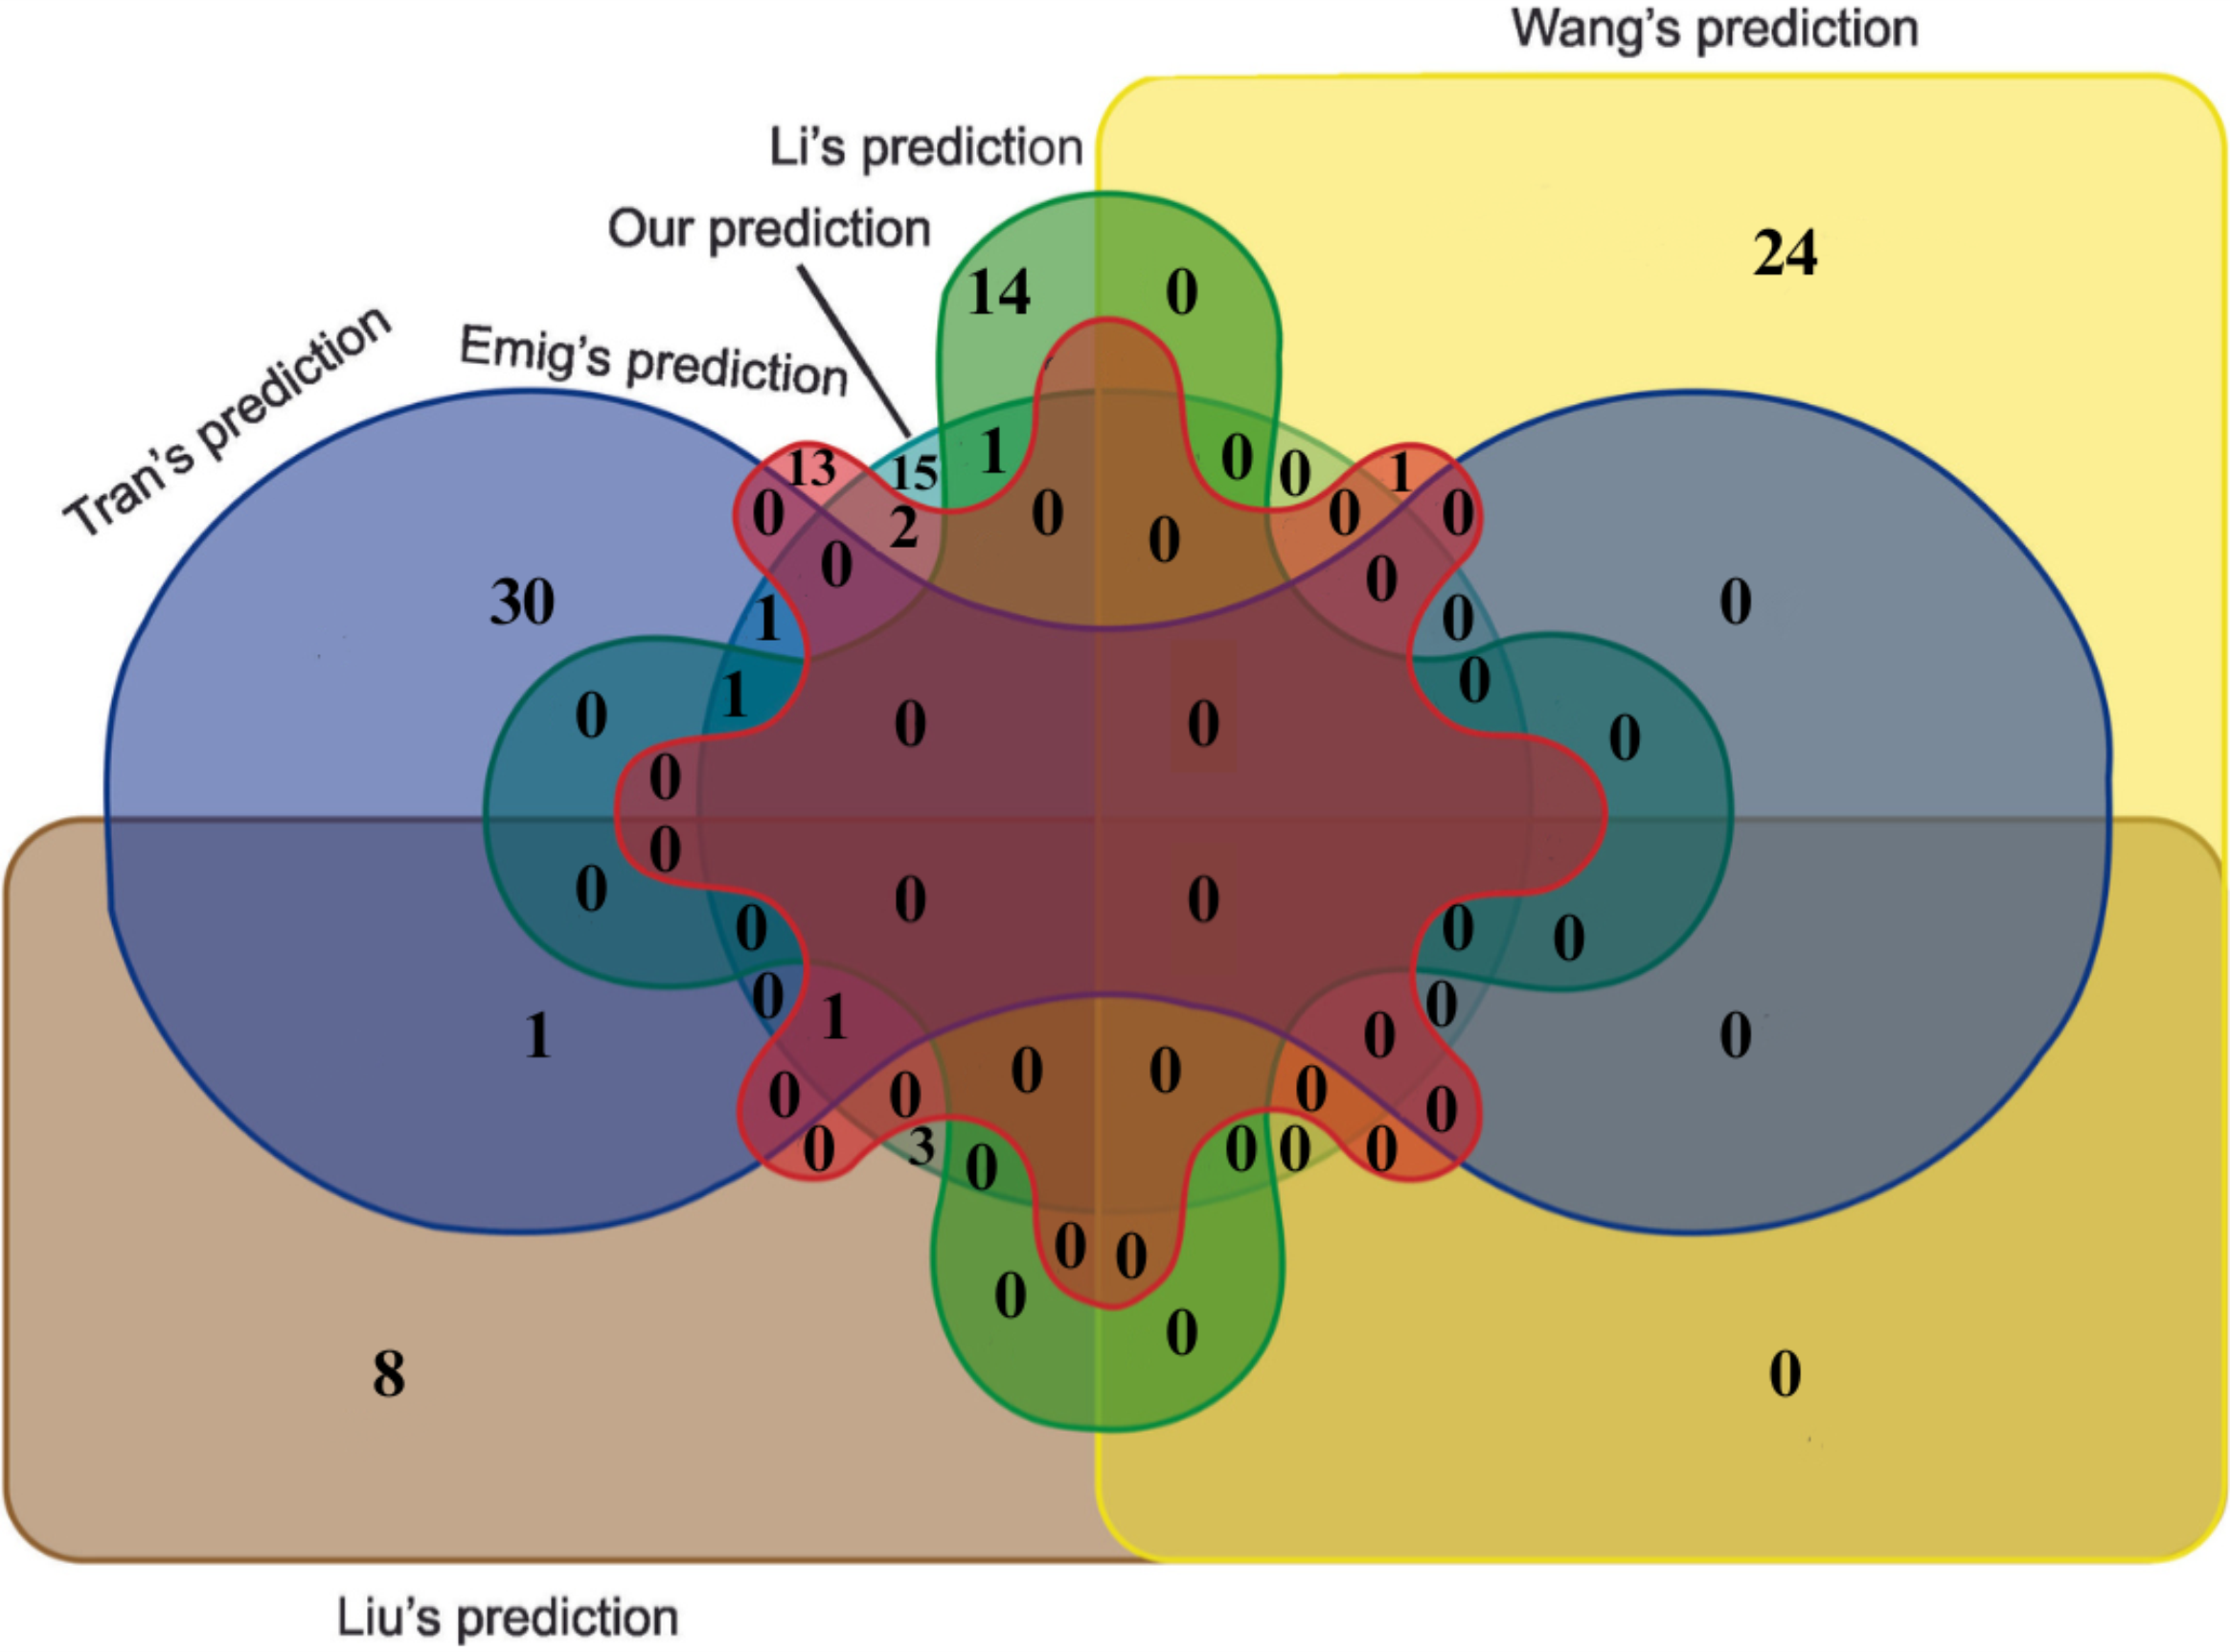
\includegraphics[scale=0.95]{images/fig2.png}
	\caption{Comparison with other predicted results.}
	\label{figure-2}
\end{figure*}

Figure 2, the Venn diagram was drawn from the predictions of five research results on anticancer drug target genes. Drivergene.net’s prediction outperforms those of the other methods, as it agrees with all other methods and gives the largest number of intersected genes. The figure was drawn with the online tool \\
www.bioinformatics.psb.ugent.be/webtools/Venn/

\section{Discussion} 
In fact, driver genes and hub genes can be significantly overlap each other in undirected networks but significantly different in directed networks. Some driver genes may serve as hub genes in undirected networks. In other words, they not only regulate key biological processes but also interact with many other genes within the network. Similarly, some hub genes may exhibit characteristics of driver genes, which exert to significantly control over network dynamics and to influence various cellular processes. The convergence of driver genes and hub genes highlights their importance in network organization and function, it can help identify key regulatory elements and potential therapeutic targets for intervention. In contrary, in directed networks, driver genes are more likely to be input nodes rather than hub nodes. For example, an input node with only a directed link to the hub node of a network can be the exact driver of the whole network because it can control the hub easily without impact from the hub node. Therefore, to exactly identify driver nodes, it cannot use network structures like centrality metrics for identification, but it should be used dynamics models like our model to locate them.\\
The study proposed a new algorithm version of the outside competitive dynamics model that can effectively execute on large-scale networks, and introduce a new software tool called Drivergene.net, an integrated approach to conveniently detecting driver nodes as well as anticancer drug target genes on large-scale networks \cite{5}. This tool allows to discovery controllability of large-scale networks, which is still in mystery up to now because of no analysis tool. First, the study proposed a software architecture to identify driver nodes in large-scale biomolecular networks, using the OpenCL library as a solution that fully exploits the computing power of multi-core CPUs. The top 10 driver genes, with the highest total support, were examined using the collected evidence on the PubMed database that proved that these genes are anticancer drug target genes. This investigation proved that the tool can work with various network types with directed, undirected, and mixed links. Second, from the proposed process and the algorithm of the outside competitive dynamics model, the study implemented the model’s algorithm and developed a Cytoscape plug-in software called Drivegene.net with three execution modes, as follows: 1) executing sequentially; 2) executing parallelly on CPUs; and 3) executing parallelly on all computing devices. Finally, the computational performance of the software tested with various sizes of large-scale biomolecular networks proved that the parallel algorithm was correctly implemented. Especially, the computation on three human large-scale biomolecular networks, including a human protein interaction network (undirected network), a human gene regulatory network (directed network), and a human signaling network (mixed network) showed that the parallel algorithm with the help of the OpenCL library provided the outstanding ability to identify driver nodes. Specifically, 86.67\% of the top 10 driver genes with the highest total support were proved as candidate anticancer drug target genes from these networks. Interestingly, the study also found that these genes are located at the innermost core of these networks. This finding is consistent with earlier studies indicating that important cancer biomarker genes are often located in the innermost core of biological networks \cite{31,32,33}, and these genes often act as anticancer drug target genes and cancer biomarkers in biological networks \cite{23}. The high consistency of these results was tested in comparison with five other prediction methods, and the predictions of Drivergene.net were better than those of competitors, as it agrees with almost other methods and provides the largest number of intersection genes. The intersection genes refer to genes encoding phosphoproteins, which are proven as biomarkers in cancer therapy. The model and software used in this study can effectively detect driver nodes from complex networks as well as anticancer drug target genes from biomolecular networks. In real life, a network system may be interacted by multiple outside agents by multiple links to the nodes inside the system. It’s hard to simulate and find driver node by this method without any improvement. In the future, it is possible to further develop the model with more than one interaction to the system at the same time. For example, in cancer therapy, combination therapies may be used simultaneously chemistry or targeted drug to inhibit driver genes in anti-cancer therapy. It is still necessary problem to solve in the future.\\

%% The Appendices part is started with the command \appendix;
%% appendix sections are then done as normal sections
%\appendix

\textbf{Authorship contribution statement}.
D.T.P. conceived the study, designed and tested the software, drafted the manuscript, revised the manuscript. T.D.T. helped conceived the study, wrote the pseudocode, revised the manuscript, guided the implement of the software, and provided guidance for the theoretical and mathematical issues and context. All authors contributed critical feedback and edited the manuscript.\\

\textbf{Declaration of competing interest}.
None \\

\textbf{Acknowledgments}.
This research was funded by Hanoi University of Industry for the research team led by the corresponding author.\\

\textbf{Supplementary data}. Supplementary data to this article can be found online at \\
https://github.com/tinhpd/Drivergene.git 

\begin{thebibliography}{71}
	\bibitem{1}
	Y.-Y. Liu, J.-J. Slotine, and A.-L. Barabási, "Controllability of complex networks," Nature, vol. 473, no. 7346, pp. 167-173, 2011/05/01 2011. https://doi.org/10.1038/nature10011
	\bibitem{2}
	J. Ruths and D. Ruths, "Control profiles of complex networks," Science, vol. 343, no. 6177, pp. 1373-1376, 2014. https://doi.org/10.1126/science.1242063
	\bibitem{3}
	T. Nepusz and T. Vicsek, "Controlling edge dynamics in complex networks," Nature Physics, vol. 8, no. 7, pp. 568-573, 2012. https://doi.org/10.1038/nphys2327
	\bibitem{4}
	W.-F. Guo, S.-W. Zhang, Q.-Q. Shi, C.-M. Zhang, T. Zeng, and L. Chen, "A novel algorithm for finding optimal driver nodes to target control complex networks and its applications for drug targets identification," BMC Genomics, vol. 19, no. 1, p. 924, 2018/01/19 2018. https://doi.org/10.1186/s12864-017-4332-z
	\bibitem{5}
	T.-D. Tran and D.-T. Pham, "Identification of anticancer drug target genes using an outside competitive dynamics model on cancer signaling networks," Scientific Reports, vol. 11, no. 1, p. 14095, 2021/07/08 2021. http://dx.doi.org/10.1038/s41598-021-93336-z.
	\bibitem{6}
	Han, Y., et al., DriverML: a machine learning algorithm for identifying driver genes in cancer sequencing studies. Nucleic Acids Res, 2019. 47(8): p. e45. https://doi.org/10.1093/nar/gkz096
	\bibitem{7}
	L. Mirsadeghi, R. Haji Hosseini, A. M. Banaei-Moghaddam, and K. Kavousi, "EARN: an ensemble machine learning algorithm to predict driver genes in metastatic breast cancer," (in eng), BMC Med Genomics, vol. 14, no. 1, p. 122, May 7 2021. http://dx.doi.org/10.1186/s12920-021-00974-3.
	\bibitem{8}
	S. J. Malebary and Y. D. Khan, "Evaluating machine learning methodologies for identification of cancer driver genes," (in eng), Scientific reports, vol. 11, no. 1, pp. 12281-12281, 2021. http://dx.doi.org/10.1038/s41598-021-91656-8.
	\bibitem{9}
	R. Andrades and M. Recamonde-Mendoza, "Machine learning methods for prediction of cancer driver genes: a survey paper," Briefings in Bioinformatics, 2022. http://dx.doi.org/10.1093/bib/bbac062.
	\bibitem{10}
	X. Hua, H. Xu, Y. Yang, J. Zhu, P. Liu, and Y. Lu, "DrGaP: a powerful tool for identifying driver genes and pathways in cancer sequencing studies," (in eng), Am J Hum Genet, vol. 93, no. 3, pp. 439-51, Sep 5 2013. http://dx.doi.org/10.1016/j.ajhg.2013.07.003.
	\bibitem{11}
	D. Tamborero, A. Gonzalez-Perez, and N. Lopez-Bigas, "OncodriveCLUST: exploiting the positional clustering of somatic mutations to identify cancer genes," (in eng), Bioinformatics, vol. 29, no. 18, pp. 2238-44, Sep 15 2013. http://dx.doi.org/10.1093/bioinformatics/btt395.
	\bibitem{12}
	T. Wang et al., "OncoVar: an integrated database and analysis platform for oncogenic driver variants in cancers," (in eng), Nucleic acids research, vol. 49, no. D1, pp. D1289-D1301, 2021. http://dx.doi.org/10.1093/nar/gkaa1033.
	\bibitem{13}
	D.-H. Le, N. Xuan Hoai, and Y.-K. Kwon, "A Comparative Study of Classification-Based Machine Learning Methods for Novel Disease Gene Prediction," in Knowledge and Systems Engineering, Cham, 2015, pp. 577-588: Springer International Publishing.
	\bibitem{14}
	A. M. Schnoes, S. D. Brown, I. Dodevski, and P. C. Babbitt, "Annotation error in public databases: misannotation of molecular function in enzyme superfamilies," (in eng), PLoS Comput Biol, vol. 5, no. 12, p. e1000605, Dec 2009. http://dx.doi.org/10.1371/journal.pcbi.1000605.
	\bibitem{15}
	Nguyen, T.-T., et al., Exploring the Molecular Terrain: A Survey of Analytical Methods for Biological Network Analysis. Symmetry, 2024. 16(4): p. 462. https://doi.org/10.3390/sym16040462
	\bibitem{16}
	X. Wang, N. Gulbahce, and H. Yu, "Network-based methods for human disease gene prediction," Briefings in Functional Genomics, vol. 10, no. 5, pp. 280-293, 2011. http://dx.doi.org/10.1093/bfgp/elr024.
	\bibitem{17}
	T.-D. Tran and Y.-K. Kwon, "Hierarchical closeness efficiently predicts disease genes in a directed signaling network," Computational Biology and Chemistry, vol. 53, pp. 191-197, 2014/12/01/ 2014. https://doi.org/10.1016/j.compbiolchem.2014.08.023.
	\bibitem{18}
	S. Erten, G. Bebek, R. M. Ewing, and M. Koyutürk, "DADA: Degree-Aware Algorithms for Network-Based Disease Gene Prioritization," (in eng), BioData Min, vol. 4, p. 19, Jun 24 2011. http://dx.doi.org/10.1186/1756-0381-4-19.
	\bibitem{19}
	A. Gottlieb, O. Magger, I. Berman, E. Ruppin, and R. Sharan, "PRINCIPLE: a tool for associating genes with diseases via network propagation," (in eng), Bioinformatics, vol. 27, no. 23, pp. 3325-6, Dec 1 2011. http://dx.doi.org/10.1093/bioinformatics/btr584.
	\bibitem{20}
	C. L. Hsu, Y. H. Huang, C. T. Hsu, and U. C. Yang, "Prioritizing disease candidate genes by a gene interconnectedness-based approach," (in eng), BMC Genomics, vol. 12 Suppl 3, no. Suppl 3, p. S25, Nov 30 2011. http://dx.doi.org/10.1186/1471-2164-12-s3-s25.
	\bibitem{21}
	X. Wu, R. Jiang, M. Q. Zhang, and S. Li, "Network-based global inference of human disease genes," (in eng), Molecular systems biology, vol. 4, pp. 189-189, 2008. http://dx.doi.org/10.1038/msb.2008.27.
	\bibitem{22}
	T. Opsahl, F. Agneessens, and J. Skvoretz, "Node centrality in weighted networks: Generalizing degree and shortest paths," Social Networks, vol. 32, no. 3, pp. 245-251, 2010/07/01/ 2010. https://doi.org/10.1016/j.socnet.2010.03.006.
	\bibitem{23}
	V. Ravindran, S. V, and G. Bagler, "Identification of critical regulatory genes in cancer signaling network using controllability analysis," Physica A: Statistical Mechanics and its Applications, vol. 474, pp. 134-143, 2017/05/15/ 2017. https://doi.org/10.1016/j.physa.2017.01.059.
	\bibitem{24}
	T.-D. Tran and Y.-K. Kwon, "Hierarchical closeness-based properties reveal cancer survivability and biomarker genes in molecular signaling networks," PLOS ONE, vol. 13, no. 6, p. e0199109, 2018. http://dx.doi.org/10.1371/journal.pone.0199109.
	\bibitem{25}
	D. Breitkreutz, L. Hlatky, E. Rietman, and J. A. Tuszynski, "Molecular signaling network complexity is correlated with cancer patient survivability," Proceedings of the National Academy of Sciences, vol. 109, no. 23, p. 9209, 2012. http://dx.doi.org/10.1073/pnas.1201416109.
	\bibitem{26}
	O. Köhler, D. V. Jarikote, I. Singh, V. S. Parmar, E. Weinhold, and O. Seitz, "Forced intercalation as a tool in gene diagnostics and in studying DNA–protein interactions," (in English), Pure and Applied Chemistry, vol. 77, no. 1, p. 327, 2005.  https://doi.org/10.1351/pac200577010327.
	\bibitem{27}
	D. H. Le and Y. K. Kwon, "Neighbor-favoring weight reinforcement to improve random walk-based disease gene prioritization," Comput Biol Chem, vol. 44, pp. 1-8, Jun 2013. http://dx.doi.org/10.1016/j.compbiolchem.2013.01.001.
	\bibitem{28}
	O. Vanunu, O. Magger, E. Ruppin, T. Shlomi, and R. Sharan, "Associating Genes and Protein Complexes with Disease via Network Propagation," PLOS Computational Biology, vol. 6, no. 1, p. e1000641, 2010. http://dx.doi.org/10.1371/journal.pcbi.1000641.
	\bibitem{29}
	C.-D. Truong, T.-D. Tran, and Y.-K. Kwon, "MORO: a Cytoscape app for relationship analysis between modularity and robustness in large-scale biological networks," BMC Systems Biology, vol. 10, no. 4, p. 122, 2016/12/23 2016. http://dx.doi.org/10.1186/s12918-016-0363-3.
	\bibitem{30}
	A. Kittas, A. Barozet, J. Sereshti, N. Grabe, and S. Tsoka, "CytoASP: a Cytoscape app for qualitative consistency reasoning, prediction and repair in biological networks," (in eng), BMC Syst Biol, vol. 9, p. 34, Jul 11 2015. http://dx.doi.org/10.1186/s12918-015-0179-6.
	\bibitem{31}
	L. Weng et al., "Identification of cyclin B1 and Sec62 as biomarkers for recurrence in patients with HBV-related hepatocellular carcinoma after surgical resection," (in eng), Molecular cancer, vol. 11, pp. 39-39, 2012. http://dx.doi.org/10.1186/1476-4598-11-39.
	\bibitem{32}
	Y. Y. Lu et al., "Transcriptional profiling and co-expression network analysis identifies potential biomarkers to differentiate chronic hepatitis B and the caused cirrhosis," (in eng), Mol Biosyst, vol. 10, no. 5, pp. 1117-25, May 2014. http://dx.doi.org/10.1039/c3mb70474b.
	\bibitem{33}
	Y. Zhang et al., "Identification of GRB2 and GAB1 coexpression as an unfavorable prognostic factor for hepatocellular carcinoma by a combination of expression profile and network analysis," (in eng), PLoS One, vol. 8, no. 12, p. e85170, 2013.
	\bibitem{34}
	T.-D. Tran and M.-T. Nguyen, "C-Biomarker. net: A Cytoscape app for the identification of cancer biomarker genes from cores of large biomolecular networks," Biosystems, p. 104887, 2023. http://dx.doi.org/10.1371/journal.pone.0085170.
	\bibitem{35}
	Q. Cui et al., "A map of human cancer signaling," (in eng), Mol Syst Biol, vol. 3, p. 152, 2007. http://dx.doi.org/10.1038/msb4100200.
	\bibitem{36}
	K.-I. Goh, M. E. Cusick, D. Valle, B. Childs, M. Vidal, and A.-L. Barabási, "The human disease network," Proceedings of the National Academy of Sciences, vol. 104, no. 21, pp. 8685-8690, 2007. http://dx.doi.org/doi:10.1073/pnas.0701361104.
	\bibitem{37}
	Z. P. Liu, C. Wu, H. Miao, and H. Wu, "RegNetwork: an integrated database of transcriptional and post-transcriptional regulatory networks in human and mouse," (in eng), Database (Oxford), vol. 2015, 2015. http://dx.doi.org/10.1093/database/bav095.
	\bibitem{38}
	P. Kong, G. Huang, and W. Liu, "Identification of protein complexes and functional modules in E. coli PPI networks," BMC Microbiology, vol. 20, no. 1, p. 243, 2020/08/06 2020. http://dx.doi.org/10.1186/s12866-020-01904-6.
	\bibitem{39}
	M. Kanehisa, M. Furumichi, M. Tanabe, Y. Sato, and K. Morishima, "KEGG: new perspectives on genomes, pathways, diseases and drugs," (in eng), Nucleic Acids Res, vol. 45, no. D1, pp. D353-d361, Jan 4 2017. http://dx.doi.org/10.1093/nar/gkw1092.
	\bibitem{40}
	M. Kanehisa, S. Goto, M. Furumichi, M. Tanabe, and M. Hirakawa, "KEGG for representation and analysis of molecular networks involving diseases and drugs," (in eng), Nucleic Acids Res, vol. 38, no. Database issue, pp. D355-60, Jan 2010.
	\bibitem{41}
	H.-C. Trinh, D.-H. Le, and Y.-K. Kwon, "PANET: A GPU-Based Tool for Fast Parallel Analysis of Robustness Dynamics and Feed-Forward/Feedback Loop Structures in Large-Scale Biological Networks," PLOS ONE, vol. 9, no. 7, p. e103010, 2014. http://dx.doi.org/10.1093/nar/gkp896.
	\bibitem{42}
	J. Concetti and C. L. Wilson, "NFKB1 and Cancer: Friend or Foe?," (in eng), Cells, vol. 7, no. 9, Sep 7 2018. http://dx.doi.org/10.3390/cells7090133.
	\bibitem{43}
	D. Verzella et al., "Life, death, and autophagy in cancer: NF-$\kappa$B turns up everywhere," (in eng), Cell Death Dis, vol. 11, no. 3, p. 210, Mar 30 2020. http://dx.doi.org/10.1038/s41419-020-2399-y.
	\bibitem{44}
	C. L. Wilson et al., "NF-$\kappa$B is a suppressor of neutrophil-driven hepatocellular carcinoma," (in eng), Nat Commun, vol. 6, p. 6818, Apr 16 2015. http://dx.doi.org/10.1038/ncomms7818.
	\bibitem{45}
	D. J. Voce et al., "Nfkb1 is a haploinsufficient DNA damage-specific tumor suppressor," (in eng), Oncogene, vol. 34, no. 21, pp. 2807-13, May 21 2015. http://dx.doi.org/10.1038/onc.2014.211.
	\bibitem{46}
	L. A. O'Reilly et al., "Loss of NF-$\kappa$B Causes Gastric Cancer with Aberrant Inflammation and Expression of Immune Checkpoint Regulators in a STAT-1-Dependent Manner," (in eng), Immunity, vol. 48, no. 3, pp. 570-583.e8, Mar 20 2018. http://dx.doi.org/10.1016/j.immuni.2018.03.003.
	\bibitem{47}
	Y. Zhou et al., "Activation of nuclear factor-kappaB (NFkappaB) identifies a high-risk subset of hormone-dependent breast cancers," (in eng), Int J Biochem Cell Biol, vol. 37, no. 5, pp. 1130-44, May 2005. http://dx.doi.org/10.1016/j.biocel.2004.09.006.
	\bibitem{48}
	A. Saccani et al., "p50 nuclear factor-kappaB overexpression in tumor-associated macrophages inhibits M1 inflammatory responses and antitumor resistance," (in eng), Cancer Res, vol. 66, no. 23, pp. 11432-40, Dec 1 2006. http://dx.doi.org/10.1158/0008-5472.can-06-1867.
	\bibitem{49}
	C. Porta et al., "Protumor Steering of Cancer Inflammation by p50 NF-$\kappa$B Enhances Colorectal Cancer Progression," (in eng), Cancer Immunol Res, vol. 6, no. 5, pp. 578-593, May 2018. http://dx.doi.org/10.1158/2326-6066.cir-17-0036.
	\bibitem{50}
	T. Hamzehloie, M. Mojarrad, M. Hasanzadeh Nazarabadi, and S. Shekouhi, "The role of tumor protein 53 mutations in common human cancers and targeting the murine double minute 2-p53 interaction for cancer therapy," (in eng), Iran J Med Sci, vol. 37, no. 1, pp. 3-8, Mar 2012.
	\bibitem{51}
	I. Goldstein, V. Marcel, M. Olivier, M. Oren, V. Rotter, and P. Hainaut, "Understanding wild-type and mutant p53 activities in human cancer: new landmarks on the way to targeted therapies," (in eng), Cancer Gene Ther, vol. 18, no. 1, pp. 2-11, Jan 2011. http://dx.doi.org/10.1038/cgt.2010.63.
	\bibitem{52}
	T. Stokłosa and J. Gołab, "Prospects for p53-based cancer therapy," (in eng), Acta Biochim Pol, vol. 52, no. 2, pp. 321-8, 2005.
	\bibitem{53}
	S. Nam et al., "Action of the Src family kinase inhibitor, dasatinib (BMS-354825), on human prostate cancer cells," (in eng), Cancer Res, vol. 65, no. 20, pp. 9185-9, Oct 15 2005. http://dx.doi.org/10.1158/0008-5472.can-05-1731.
	\bibitem{54}
	M. Goldenberg-Furmanov et al., "Lyn is a target gene for prostate cancer: sequence-based inhibition induces regression of human tumor xenografts," (in eng), Cancer Res, vol. 64, no. 3, pp. 1058-66, Feb 1 2004. http://dx.doi.org/10.1158/0008-5472.can-03-2420.
	\bibitem{55}
	J. B. Bolen, N. Rosen, and M. A. Israel, "Increased pp60c-src tyrosyl kinase activity in human neuroblastomas is associated with amino-terminal tyrosine phosphorylation of the src gene product," (in eng), Proc Natl Acad Sci U S A, vol. 82, no. 21, pp. 7275-9, Nov 1985. http://dx.doi.org/10.1073/pnas.82.21.7275.
	\bibitem{56}
	A. N. Shah and G. E. Gallick, "Src, chemoresistance and epithelial to mesenchymal transition: are they related?," (in eng), Anticancer Drugs, vol. 18, no. 4, pp. 371-5, Apr 2007. http://dx.doi.org/10.1097/CAD.0b013e32801265d7.
	\bibitem{57}
	M. S. Duxbury, H. Ito, M. J. Zinner, S. W. Ashley, and E. E. Whang, "siRNA directed against c-Src enhances pancreatic adenocarcinoma cell gemcitabine chemosensitivity," (in eng), J Am Coll Surg, vol. 198, no. 6, pp. 953-9, Jun 2004. http://dx.doi.org/10.1016/j.jamcollsurg.2004.01.037.
	\bibitem{58}
	C. Jacobs and H. Rübsamen, "Expression of pp60c-src protein kinase in adult and fetal human tissue: high activities in some sarcomas and mammary carcinomas," (in eng), Cancer Res, vol. 43, no. 4, pp. 1696-702, Apr 1983.
	\bibitem{59}
	S. Vemulapalli et al., "Phase I open-labeled trial of gemcitabine and dasatinib in advanced solid tumors," Journal of Clinical Oncology, vol. 26, no. 15 suppl, pp. 14626-14626, 2008.
	\bibitem{60}
	G. Giaccone and P. Zucali, "Src as a potential therapeutic target in non-small-cell lung cancer," Annals of Oncology, vol. 19, no. 7, pp. 1219-1223, 2008.
	\bibitem{61}
	W. Wang, F. Liu, C. Wang, C. Wang, Y. Tang, and Z. Jiang, "Src Promotes Metastasis of Human Non-Small Cell Lung Cancer Cells through Fn14-Mediated NF-$\kappa$B Signaling," (in eng), Med Sci Monit, vol. 24, pp. 1282-1294, Mar 3 2018. http://dx.doi.org/10.12659/msm.906266.
	\bibitem{62}
	F. M. Johnson, B. Saigal, M. Talpaz, and N. J. Donato, "Dasatinib (BMS-354825) tyrosine kinase inhibitor suppresses invasion and induces cell cycle arrest and apoptosis of head and neck squamous cell carcinoma and non-small cell lung cancer cells," (in eng), Clin Cancer Res, vol. 11, no. 19 Pt 1, pp. 6924-32, Oct 1 2005. http://dx.doi.org/10.1158/1078-0432.ccr-05-0757.
	\bibitem{63}
	P. Koppikar et al., "Combined inhibition of c-Src and epidermal growth factor receptor abrogates growth and invasion of head and neck squamous cell carcinoma," (in eng), Clin Cancer Res, vol. 14, no. 13, pp. 4284-91, Jul 1 2008. http://dx.doi.org/10.1158/1078-0432.ccr-07-5226.
	\bibitem{64}
	M. P. Lutz et al., "Overexpression and activation of the tyrosine kinase Src in human pancreatic carcinoma," (in eng), Biochem Biophys Res Commun, vol. 243, no. 2, pp. 503-8, Feb 13 1998. http://dx.doi.org/10.1006/bbrc.1997.8043.
	\bibitem{65}
	J. M. Summy and G. E. Gallick, "Treatment for advanced tumors: SRC reclaims center stage," (in eng), Clin Cancer Res, vol. 12, no. 5, pp. 1398-401, Mar 1 2006. http://dx.doi.org/10.1158/1078-0432.ccr-05-2692.
	\bibitem{66}
	J. Du et al., "Bead-based profiling of tyrosine kinase phosphorylation identifies SRC as a potential target for glioblastoma therapy," (in eng), Nat Biotechnol, vol. 27, no. 1, pp. 77-83, Jan 2009. http://dx.doi.org/10.1038/nbt.1513.
	\bibitem{67}
	X. Wang and R. Simon, "Identification of potential synthetic lethal genes to p53 using a computational biology approach," BMC Medical Genomics, vol. 6, no. 1, p. 30, 2013/09/11 2013. http://dx.doi.org/10.1186/1755-8794-6-30.
	\bibitem{68}
	D. Emig et al., "Drug Target Prediction and Repositioning Using an Integrated Network-Based Approach," PLOS ONE, vol. 8, no. 4, p. e60618, 2013. http://dx.doi.org/10.1371/journal.pone.0060618.
	\bibitem{69}
	C. Li et al., "Cancer-Drug Interaction Network Construction and Drug Target Prediction Based on Multi-source Data," in Wireless Algorithms, Systems, and Applications, Cham, 2018, pp. 223-235: Springer International Publishing.
	\bibitem{70}
	L. Liu et al., "Synthetic Lethality-based Identification of Targets for Anticancer Drugs in the Human Signaling Network," Scientific Reports, vol. 8, no. 1, p. 8440, 2018/05/31 2018. http://dx.doi.org/10.1038/s41598-018-26783-w.
	\bibitem{71}
	A. M. Carter et al., Phosphoprotein-based biomarkers as predictors for cancer therapy, Proceedings of the National Academy of Sciences, vol. 117, no. 31, pp. 18401-18411, 2020. http://dx.doi.org/doi:10.1073/pnas.2010103117.
\end{thebibliography}
\end{document}

\endinput
%%
%% End of file `elsarticle-template-num.tex'.
